
\section{Equations for incompressible fluids}

Roughly-speaking, a \emph{fluid} is a mathematical abstraction in which the density and the velocity of a mass of particles are given by continuous functions.  We present only enough of the theory of fluids to give an example of solving the Stokes model for slow, very-viscous fluids, and we keep to the constant-density case.  A comprehensive introduction to modeling of fluids, from \citep{Acheson1990} or \citep{Fowler1997} for example, is recommended.

Consider an incompressible fluid with velocity $\bu=\bu(t,x,y,z)$, of constant density $\rho$, with \emph{(dynamic) viscosity} $\mu$, and subject to a \emph{body force} $\rho \bg$ where $\bg$ has units of acceleration.  The incompressible variable-viscosity \emph{Navier-Stokes model} has these main equations
\begin{align}
\rho \left(\frac{\partial \bu}{\partial t} + \bu \cdot \grad \bu\right) &= \Div \sigma + \rho \bg, \label{eq:ok:nsmomentum} \\
\Div \bu &= 0, \label{eq:ok:nsincomp} \\
\sigma &= 2 \mu\, D \bu - p I. \label{eq:ok:nsflowlaw}
\end{align}
Equation \eqref{eq:ok:nsmomentum} is an equation of \emph{momentum conservation} (or \emph{balance}), which is to say a statement of Newton's second law ``$ma=F$,'' and \eqref{eq:ok:nsincomp} states incompressibility.  The \emph{flow law} \eqref{eq:ok:nsflowlaw} relates the stress tensor $\sigma=\sigma_{ij}$ to the \emph{strain rate tensor}, the symmetrized velocity gradient
    $$D \bu = \frac{1}{2} \left(\grad \bu + \grad \bu^{\top}\right).$$
Because of the symmetry of the stress and strain-rate tensors, equations \eqref{eq:ok:nsmomentum}, \eqref{eq:ok:nsincomp}, \eqref{eq:ok:nsflowlaw} represent $3+1+6=10$ scalar equations, respectively.

Our notation has hit a ``subscripting crisis'', so we use a superscript for components of the velocity field, namely $\bu = \left<u^x,u^y,u^z\right>$.  In this notation the spatial derivatives in the above equations are, by definition,
\begin{equation}
\grad \bu = \renewcommand{\arraystretch}{1.3}\begin{bmatrix}
    \frac{\partial u^x}{\partial x} & \frac{\partial u^y}{\partial x} & \frac{\partial u^z}{\partial x} \\
    \frac{\partial u^x}{\partial y} & \frac{\partial u^y}{\partial y} & \frac{\partial u^z}{\partial y} \\
    \frac{\partial u^x}{\partial z} & \frac{\partial u^y}{\partial z} & \frac{\partial u^z}{\partial z}
    \end{bmatrix}, \quad
\Div \bu = \frac{\partial u^x}{\partial x} + \frac{\partial u^y}{\partial y} + \frac{\partial u^z}{\partial z}. \label{eq:ok:graddivudefinition}
\end{equation}

To give some additional physical meaning to equations \eqref{eq:ok:nsmomentum}--\eqref{eq:ok:nsflowlaw}, if we measure distances in meters, mass in kilograms, and time in seconds (``MKS units'') then the quantities which are balanced in \eqref{eq:ok:nsmomentum} are in units $\text{kg}\, \text{m}^{-2}\, \text{s}^{-2}$, namely \emph{stress gradients}.  In fact, noting that the MKS unit of force is the Newton ($\text{N}=\text{kg}\, \text{m}\, \text{s}^{-2}$), the quantities in \eqref{eq:ok:nsmomentum} are forces per unit area, or stress in Pascals ($\text{Pa} = \text{N}\, \text{m}^{-2}$) per meter.  The velocity derivatives $\grad \bu$ and $D\bu$ have units of $\text{s}^{-1}$ and the dynamic viscosity $\mu$ has units $\text{Pa}\, \text{s} = \text{kg}\, \text{m}^{-1}\, \text{s}^{-1}$.

FIXME: theory where Froude $\approx 0$

In the \emph{(variable-viscosity) Stokes model} the body force, the pressure gradient, and the viscous stress gradients are in balance.  This is the model which arises when we set the entire acceleration term on the left side of \eqref{eq:ok:nsmomentum} to zero:
\begin{align}
- \Div \left(\mu \left(\grad \bu + \grad \bu^{\top}\right)\right) + \grad p &= \rho \bg \label{eq:ok:varstokesmomentum} \\
\Div \bu &= 0 \label{eq:ok:varstokesincomp}
\end{align}
A shallow case of these equations will be addressed in Chapter \ref{chap:co}, with a nontrivial model for the variable viscosity $\mu$.

In the current Chapter, however, we consider the case where the viscosity $\mu$ is constant.  In such case the velocity second derivative term is a Laplacian operator (Exercise \ref{chap:ok}.\ref{exer:ok:constantviscositystokes}).  Thus for this Chapter the Stokes equations are
\begin{align}
- \mu \grad^2 \bu + \grad p &= \rho \bg  \label{eq:ok:constantviscositystokes} \\
\Div \bu &= 0  \label{eq:ok:constantviscosityincomp}
\end{align}
This is a Poisson-like problem for $\bu$, but with pressure as an additional unknown and with an additional equation stating incompressiblity.


\section{Weak form of the Stokes equations}

FIXME: theory from \citep{Braess2007,Elmanetal2005}; derive quickly

We assume that the boundary is decomposed disjointly, $\partial\Omega = \partial_D\Omega \cup \partial_N\Omega$, and on these portions we will allow (arbitrary) Dirichlet and Neumann boundary conditions.  The former correspond to having the velocity $\bu$ equal to a known function.  The derivation of the weak form, as follows, establishes the form of the latter.

Suppose $\bu$, $p$ are (classical) solutions to \eqref{eq:ok:constantviscositystokes}, \eqref{eq:ok:constantviscosityincomp}.  Suppose $\bv$, a smooth velocity test function, satisfies $\bv=0$ on $\partial_D\Omega$.  Multiplying \eqref{eq:ok:constantviscositystokes} by $\bv$ and integrating-by-parts we get
\begin{equation}
\int_{\partial_N \Omega} \left[- \mu \frac{\partial \bu}{\partial n} + p \bn \right] \cdot \bv + \int_\Omega \mu \grad \bu : \grad \bv - p \Div \bv = \int_\Omega \rho \bg \cdot \bv, \label{eq:ok:weakstokeswithboundary}
\end{equation}
where $\bn$ denotes the outward normal unit vector field on $\partial \Omega$, which we assume is adequately smooth.  See Exercise \ref{exer:ok:weakderive} for notation and additional details.

The quantity in square brackets in \eqref{eq:ok:weakstokeswithboundary} has units of stress, and we assume it is equal to a known function on the Neumann part of the boundary:
\begin{equation}
\sigma\cdot \bn = \mu \frac{\partial \bu}{\partial n} - p \bn = \bbf_N \quad \text{on } \partial_N \Omega.  \label{eq:ok:neumannbc}
\end{equation}

Define
\begin{equation}
\mathcal{V}_D = \left\{\bw \in W^{1,2}(\Omega)^3 \,\Big|\, \bw = \bbf_D \, \text{ on } \partial_D \Omega\right\}. \label{eq:ok:dirichletbc}
\end{equation}
We say $\bu \in \mathcal{V}_D$ and $p \in L^2(\Omega)$ solve the \emph{weak form of the Stokes equations} if
\begin{align}
\int_\Omega \mu \grad \bu : \grad \bv - p \Div \bv &= \int_\Omega \rho \bg \cdot \bv + \int_{\partial_N \Omega} \bbf_N \cdot \bv \label{eq:ok:weakstokesvelocity} \\
\int_\Omega q \Div \bu &= 0 \label{eq:ok:weakstokespressure}
\end{align}
for all $\bv \in \mathcal{V}_0 = W_0^{1,2}(\Omega)^3$ and $q \in L^2(\Omega)$.


\section{Example I: A small step}

Before constructing a convergent FEM for the differential equations above, which is nontrivial, let us build a small, concrete case \emph{by hand} from a very coarse grid.  This will guide our expectations about the form of the discrete equations, and it will help us think.  It will also expose the need for compatibility between the FEM spaces for velocity and pressure.

We consider a two-dimensional ``Poiseuille flow'' \citep{Acheson1990,Elmanetal2005} on $\Omega=(-1,1)\times(-1,1)$ with constant viscosity $\mu=1$ and no body force $\rho \bg=0$ (Figure \ref{fig:ok:poiseuillesolutions}).  On the left side $x=-1$ we have a Dirichlet in-flow boundary condition $\bu = \left<1-y^2,0\right>$.  On the right side $x=+1$ we choose a homogeneous Neumann (``stress-free'') boundary condition $\partial \bu/\partial n - \bn p = 0$.  On $y=\pm 1$ boundaries we have homogeneous Dirichlet (``no-slip'') boundary conditions $\bu=\left<0,0\right>$. 

\begin{figure}
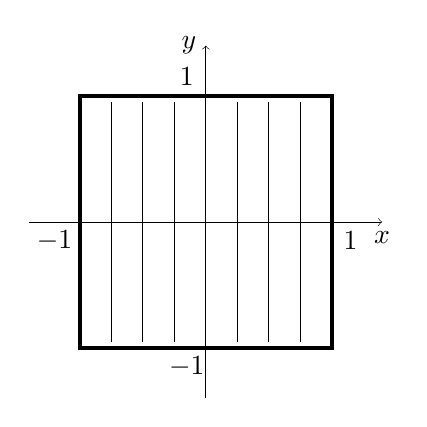
\begin{tikzpicture}[scale=1.6]
    % axes
    \draw[->,very thin] (-1.4,0.0) -- (1.4,0.0) node[below] {$x$};
    \draw[->,very thin] (0.0,-1.4) -- (0.0,1.4) node[left] {$y$};
    \node at (1.15,-0.15) {$1$};
    \node at (-1.2,-0.15) {$-1$};
    \node at (-0.15,1.15) {$1$};
    \node at (-0.15,-1.15) {$-1$};
    % domain
    \draw[line width=1.5pt] (-1,-1) -- (1,-1) -- (1,1) -- (-1,1) -- cycle;
    % contours of pressure
    \foreach \x in {-0.75, -0.5, -0.25, 0.0, 0.25, 0.5, 0.75} {
        \draw[thin]  (\x, -0.95) -- (\x,0.95);
    }
\end{tikzpicture}
\quad
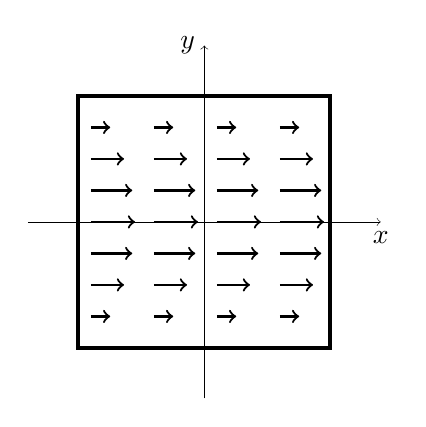
\begin{tikzpicture}[scale=1.6]
    % axes
    \draw[->,very thin] (-1.4,0.0) -- (1.4,0.0) node[below] {$x$};
    \draw[->,very thin] (0.0,-1.4) -- (0.0,1.4) node[left] {$y$};
    % domain
    \draw[line width=1.5pt] (-1,-1) -- (1,-1) -- (1,1) -- (-1,1) -- cycle;
    % velocity field as arrows
    \foreach \x in {-0.9, -0.4, 0.1, 0.6} {
        \foreach \y in {-0.75, -0.5, -0.25, 0.0, 0.25, 0.5, 0.75} {
            %\fill (\x,\y) circle[radius=1pt];
            \draw[->,thick]  (\x, \y) -- ({\x+0.35*(1.0-\y*\y)},\y);
        }
    }
\end{tikzpicture}


\caption{In a Poiseuille flow viscous shear forces from vertical variation in the velocity $\bu$ (left) are balanced by the gradient of the pressure $p$ (right; contours of constant pressure).}
\label{fig:ok:poiseuillesolutions}
\end{figure}

The fluid problem we have in mind has an exact, steady solution,
\begin{equation}
u^x = 1-y^2, \quad u^y=0, \quad p = -2(x-1).  \label{eq:ok:poiseuilleexact}
\end{equation}
This strictly-horizontal flow is driven, or balanced, by a horizontal pressure gradient.  This pressure gradient is balanced by viscous forces arising from the variation in $y$ of the $u^x$, that is, by ``shearing'' motion.

The grid in Figure \ref{fig:ok:poiseuilletinygrid}, with nine nodes and four elements, is already complicated enough because we will work-out the details by hand.  Consider functions which are minimally smooth for the weak formation \eqref{eq:ok:weakstokesvelocity}, \eqref{eq:ok:weakstokespressure}.  Specifically, let $u^x,u^y$ be from the $Q^1$ (bilinear) FEM space, as in Chapter \ref{chap:of}, and $p$ from $P^0$, the space of functions which are piecewise-constant on each element.  Thus the velocity functions are continuous, and in $W^{1,2}(\Omega)^2$, while the pressure functions are discontinuous but in $L^2(\Omega)$.

\begin{figure}
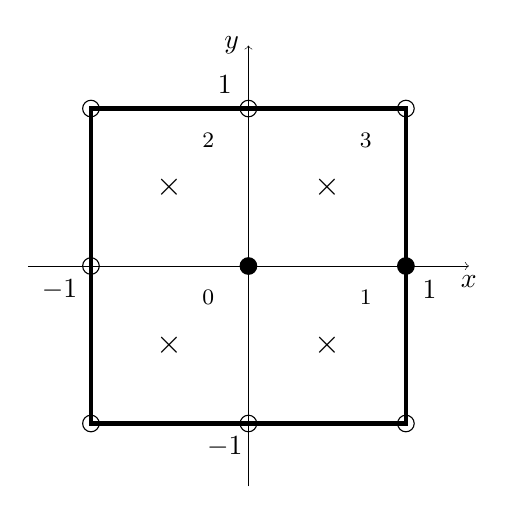
\begin{tikzpicture}[scale=2.0]
% axes
  \draw[->,very thin] (-1.4,0.0) -- (1.4,0.0) node[below] {$x$};
  \draw[->,very thin] (0.0,-1.4) -- (0.0,1.4) node[left] {$y$};
  \node at (1.15,-0.15) {$1$};
  \node at (-1.2,-0.15) {$-1$};
  \node at (-0.15,1.15) {$1$};
  \node at (-0.15,-1.15) {$-1$};
% domain and elements
  \draw[line width=1.5pt] (-1,-1) -- (1,-1) -- (1,1) -- (-1,1) -- cycle;
  \node at (-0.25,-0.2) {\large $\square_0$};
  \node at (0.75,-0.2) {\large $\square_1$};
  \node at (-0.25,0.8) {\large $\square_2$};
  \node at (0.75,0.8) {\large $\square_3$};
% velocity unknowns
  \filldraw (0.0,0.0) circle (1.5pt);
  \filldraw (1.0,0.0) circle (1.5pt);
% Dirichlet nodes
  \draw (-1.0,-1.0) circle (1.5pt);
  \draw (-1.0,0.0) circle (1.5pt);
  \draw (-1.0,1.0) circle (1.5pt);
  \draw (0.0,-1.0) circle (1.5pt);
  \draw (0.0,1.0) circle (1.5pt);
  \draw (1.0,-1.0) circle (1.5pt);
  \draw (1.0,1.0) circle (1.5pt);
% pressure unknowns
  \node at (-0.5,-0.5) {\large $\times$};
  \node at (-0.5,0.5) {\large $\times$};
  \node at (0.5,-0.5) {\large $\times$};
  \node at (0.5,0.5) {\large $\times$};
\end{tikzpicture}


\caption{Domain $\Omega=(-1,1)\times(-1,1)$ with a coarse grid of four elements $\square_k$.  Solid ``$\bullet$'' nodes are velocity unknowns, open circles ``{\large $\circ$}'' are velocity (Dirichlet) boundary conditions, and ``$\times$'' are pressure unknowns.}
\label{fig:ok:poiseuilletinygrid}
\end{figure}

Because of boundary conditions and other choices, the weak form (continuum) Poiseuille problem is
\begin{equation}
\int_\Omega \grad \bu : \grad \bv - p \Div \bv = 0, \qquad
\int_\Omega q \Div \bu = 0 \label{eq:ok:smallstokesboth}
\end{equation}
for test functions $\bv,q$.  To build the corresponding discrete FEM system, for the grid shown in Figure \ref{fig:ok:poiseuilletinygrid}, trial functions $\bu,p$ are needed.  The six nodes on $y=\pm 1$ correspond to homogeneous Dirichlet conditions $\bu=0$.  Letting $\psi_{-1},\psi_0,\psi_1$ denote $Q^1$ hat functions (Figure \ref{fig:of:q1hat}) at points $(x,y)=(-1,0),(0,0),(1,0)$, respectively, the non-homogeneous Dirichlet node at $(-1,0)$ is incorporated into the solution by the expression
\begin{equation} 
\bu = \left<\psi_{-1}+\alpha_0\psi_0+\alpha_1\psi_1,\beta_0\psi_0+\beta_1\psi_1\right>. \label{eq:ok:smallexpansionvelocity}
\end{equation}
(Because the boundary data is interpolated, this trial function is only ``approximately in'' $\mathcal{V}_D$.)  On the other hand, the pressure is expanded in $P^0$ basis functions, namely characteristic functions $\one_j = \one_{\square_j}$:
\begin{equation}
p = \gamma_0 \one_0 + \gamma_1 \one_1 + \gamma_2 \one_2 + \gamma_3 \one_3.  \label{eq:ok:smallexpansionpressure}
\end{equation}
In summary there are four velocity ($\alpha_0,\beta_0,\alpha_1,\beta_1$) and four pressure ($\gamma_0,\gamma_1,\gamma_2,\gamma_3$) degrees of freedom.

Inserting \eqref{eq:ok:smallexpansionvelocity} and \eqref{eq:ok:smallexpansionpressure} into \eqref{eq:ok:weakstokesvelocity} gives
\begin{align}
&\alpha_0 \int_\Omega \grad \psi_0 \cdot \grad v^x + \beta_0 \int_\Omega \grad \psi_0 \cdot \grad v^y \label{eq:ok:smallconcretevelocity} \\
&\qquad + \alpha_1 \int_\Omega \grad \psi_1 \cdot \grad v^x + \beta_1 \int_\Omega \grad \psi_1 \cdot \grad v^y \notag \\
&\qquad - \gamma_0 \int_{\square_0} \Div \bv - \gamma_1 \int_{\square_1} \Div \bv - \gamma_2 \int_{\square_2} \Div \bv - \gamma_3 \int_{\square_3} \Div \bv \notag \\
&= - \int_\Omega \grad \psi_{-1} \cdot \grad v^x \notag
\end{align}
for test functions $\bv \in W_0^{1,2}(\Omega)^2$.  Inserting \eqref{eq:ok:smallexpansionvelocity} into \eqref{eq:ok:weakstokespressure}, and changing the sign to give symmetry (see below), gives
\begin{align}
&- \alpha_0 \int_\Omega q \frac{\partial \psi_0}{\partial x} - \beta_0 \int_\Omega q \frac{\partial \psi_0}{\partial y} - \alpha_1 \int_\Omega q \frac{\partial \psi_1}{\partial x} - \beta_1 \int_\Omega q \frac{\partial \psi_1}{\partial y}  \label{eq:ok:smallconcretepressure} \\
&= \int_\Omega q \frac{\partial \psi_{-1}}{\partial x} \notag
\end{align}
for test functions $q \in L^2(\Omega)$.

As noted, there are eight unknown scalars in system \eqref{eq:ok:smallconcretevelocity}, \eqref{eq:ok:smallconcretepressure}.  So we choose four velocity test functions from the basis of $Q^1$ hat functions at locations of velocity unknowns,
\begin{equation}
\bv_i \in \left\{\left<\psi_0,0\right>, \left<0,\psi_0\right>, \left<\psi_1,0\right>, \left<0,\psi_1\right>\right\},  \label{eq:ok:smallvelocitytest}
\end{equation}
and four pressure test functions from a $P^0$ basis,
\begin{equation}
q_i \in \{\one_0,\one_1,\one_2,\one_3\}.  \label{eq:ok:smallpressuretest}
\end{equation}
By using \eqref{eq:ok:smallvelocitytest}, \eqref{eq:ok:smallpressuretest} in equations \eqref{eq:ok:smallconcretevelocity}, \eqref{eq:ok:smallconcretepressure} we get an $N=8$ dimensional matrix problem:
\begin{equation}
\begin{bmatrix}
r   &     & t   &     & b_0 & b_1 & b_2 & b_3 \\
    & r   &     & t   & c_0 & c_1 & c_2 & c_3 \\
t   &     & s   &     &     & d_1 &     & d_3 \\
    & t   &     & s   &     & e_1 &     & e_3 \\
b_0 & c_0 &     &     \\
b_1 & c_1 & d_1 & e_1 \\
b_2 & c_2 &     &     \\
b_3 & c_3 & d_3 & e_3
\end{bmatrix} 
\begin{bmatrix}
\alpha_0 \\ \beta_0 \\ \alpha_1 \\ \beta_1 \\ \gamma_0 \\ \gamma_1 \\ \gamma_2 \\ \gamma_3
\end{bmatrix}
=
\begin{bmatrix}
r_0 \\
0 \\
0 \\
0 \\
s_0 \\
0 \\
s_2 \\
0
\end{bmatrix}.  \label{eq:ok:smallmatrixproblem}
\end{equation} 
All blank entries are zero.  Exercise \ref{chap:ok}.\ref{exer:ok:smalldetails} describes how to compute the non-zero entries.

The system is obviously in symmetric, block form
\begin{equation}
\begin{bmatrix}
A & B^\top \\
B &
\end{bmatrix} 
\begin{bmatrix}
\bu^h \\ \bp^h
\end{bmatrix}
=
\begin{bmatrix}
\br \\
\bs
\end{bmatrix}.  \label{eq:ok:smallblockform}
\end{equation}
Based on the results of Exercise \ref{chap:ok}.\ref{exer:ok:smalldetails}, we have concretely that
    $$A = \frac{1}{3} \begin{bmatrix}
     8 &    & -1 &    \\
       &  8 &    & -1 \\
    -1 &    &  4 &    \\
       & -1 &    &  4
    \end{bmatrix},
    \quad
    B = \frac{1}{2} \begin{bmatrix}
     FIXME
    \end{bmatrix}.$$
FIXME  this gives a solvable system (sort of by accident)


\section{Example II: A stumble}

FIXME \emph{enclose} with Dirichlet outflow matching inflow; observe compatibility required (\citep{Elmanetal2005} (5.4)) but satisfied; gives $B \in \RR^{4\times 2}$ for which $B^\top$ has two-dimensional null space instead of $\Null(B^\top) = \left<\mathbf{1}\right>$ as it is supposed to; see \citep{Elmanetal2005} (5.47) and (5.64)



\clearpage
\newpage
\section{Fluid flowing down a slope}

The particular problems we will solve in \texttt{stokes.c} are the above Poiseuille flow problem (FIXME see Exercise) and additionally a constant-thickness flow down a slope of angle $\theta$, using rotated coordinates as in Figure \ref{fig:ok:slabonslope}.  The weak form is \eqref{eq:ok:weakstokesvelocity}, \eqref{eq:ok:weakstokespressure} in 2D with $\bg = (g\sin\theta,-g\cos\theta)$ for $g>0,\theta\in(-\pi/2,\pi/2)$ fixed.

\begin{marginfigure}
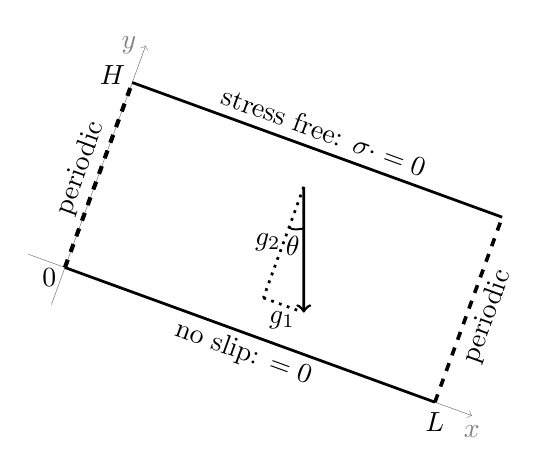
\begin{tikzpicture}[scale=2.5,rotate=-20]
  \draw[->,gray,very thin] (-0.2,0.0) -- (2.2,0.0) node[below] {$x$};
  \draw[->,gray,very thin] (0.0,-0.2) -- (0.0,1.2) node[left] {$y$};
  \node[xshift=-0.2cm,yshift=-0.13cm] at (0.0,0.0) {$0$};
  \node[xshift=0.0cm,yshift=-0.25cm] at (2.0,0.0) {$L$};
  \node[xshift=-0.25cm,yshift=0.1cm] at (0.0,1.0) {$H$};
  \draw[line width=1.0pt] (0.0,0.0) -- (2.0,0.0);
  \draw[line width=1.0pt] (0.0,1.0) -- (2.0,1.0);
  \node[rotate=-20] at (1.0,-0.1) {no slip: $\bu=0$};
  \node[rotate=-20] at (1.0,1.1) {stress free: $\sigma\cdot\bn=0$};
  \draw[line width=1.5pt,dashed] (0.0,0.0) -- (0.0,1.0);
  \draw[line width=1.3pt,dashed] (2.0,0.0) -- (2.0,1.0);
  \node[rotate=70] at (-0.1,0.5) {periodic};
  \node[rotate=70] at (2.1,0.5) {periodic};
  \draw[line width=1.0pt,dotted] (1.0,0.8) -- node[xshift=-0.2cm,yshift=0.0cm] {$g_2$} (1.0,0.2);
  \draw[line width=1.0pt,dotted] (1.0,0.2) -- node[xshift=0.0cm,yshift=-0.2cm] {$g_1$} (1.2,0.2);
  %>> 0.6 * tan((pi/180)*20)
  %ans =  0.21838
  \draw[->,line width=1.0pt] (1.0,0.8) -- (1.21838,0.2) node[xshift=0.2cm,yshift=0.6cm] {$\bg$};
  \draw[line width=0.7pt] (1.0,0.58) .. controls (1.03,0.575) and (1.04,0.585) .. (1.07,0.6);
  \node at (1.05,0.5) {$\theta$};
\end{tikzpicture}


\caption{Geometry and boundary conditions of our first Stokes problem, for a rectangular block flowing and sliding down a slope.  ``Slip'' is $\bt \cdot \sigma \cdot \bn$ given, where $\bt$ ranges over tangential vectors.  ``Non-penetration'' is $\bu\cdot\bn=0$.}
\label{fig:ok:slabonslope}
\end{marginfigure}

The domain is the rectangle $[0,L]\times[0,H]$ (in the rotated coordinates), where $H$ is the thickness and $L$ the length.  We assume a stress-free top and no penetration at the base.  FIXME  Because the normal direction to the top is in the (rotated) $y$-direction, the top boundary condition is
  $$\sigma\cdot\bn = 0 \iff
\begin{bmatrix}
2 \mu u_x - p & \mu (u_y+v_x) \\
\mu (u_y+v_x) & 2 \mu v_y - p
\end{bmatrix} \begin{bmatrix}
0 \\ 1
\end{bmatrix} = \begin{bmatrix}
0 \\ 0
\end{bmatrix}.$$
Thus, with the no-slip base, we have these boundary conditions,
\begin{align}
\text{top $y=H$:}&    & &\begin{array}{l} u_y + v_x = 0 \\ 2 \mu v_y = p\end{array}  \label{eq:ok:bcstokestop} \\
\text{bottom $y=0$:}& & &\begin{array}{l} u = 0 \\ v = 0 \end{array} \label{eq:ok:bcstokesbottom}
\end{align}

FIXME: make exercise.  This boundary-value problem has a well-known exact solution in the no-slip case, which makes this a good example for our first numerical approach:
\begin{align}
u &= \frac{\rho g_1}{\mu} y \left(H - \frac{y}{2}\right), \label{eq:ok:exactstokesu} \\
v &= 0, \label{eq:ok:exactstokesv} \\
p &= - \rho g_2 (H-y).\label{eq:ok:exactstokesp}
\end{align}


\clearpage
\newpage
\section{Finite element, structured-grid approach}

In this section we apply FIXME to get a symmetric linear system
\begin{equation}
  A \bz = \bbf \label{eq:ok:linsysstokes}
\end{equation}
with block structure FIXME.  As usual we treat the linear problem as nonlinear, and we use a structured grid, so our code has a \pSNES and \pDMDA objects.  We first provide a residual-evaluation routine for the locally-owned part of the structured grid.


\section{A stable $Q^2-P^{-1}$ FEM}

FIXME:  write \texttt{stokes.c} here


\section{Preconditioners for indefinite systems}

FIXME: while $A$ is symmetric, it is not positive definite; note that if
    $$M = \begin{bmatrix} 0 & G \\ G^\top & 0 \end{bmatrix}$$
and if $M$ has eigenvalue $\lambda$ so that
    $$M \begin{bmatrix} \bx \\ \by \end{bmatrix} = \lambda \begin{bmatrix} \bx \\ \by \end{bmatrix}$$
then
    $$M \begin{bmatrix} -\bx \\ \by \end{bmatrix} = - \lambda \begin{bmatrix} -\bx \\ \by \end{bmatrix}$$
and (w.o.l.o.g.) this is a lin.-indep. eigenvector so $M$ also has eigenvalue $-\lambda$


\section{Exercises}

\renewcommand{\labelenumi}{\arabic{chapter}.\arabic{enumi}\quad}
\begin{enumerate}

\item \label{exer:ok:constantviscositystokes}  Starting from \eqref{eq:ok:graddivudefinition}, by commuting mixed derivatives and using incompressibility show that
\begin{equation*}
\Div \left(\grad \bu^{\top}\right) = \begin{bmatrix}
    \frac{\partial}{\partial x}\left(\Div \bu\right) & \frac{\partial}{\partial y }\left(\Div \bu\right) & \frac{\partial}{\partial x} \left(\Div \bu\right)
    \end{bmatrix}
    = 0.
\end{equation*}
On the other hand,
\begin{equation*}
\Div \left(\grad \bu\right) = \begin{bmatrix} \grad^2 u^x & \grad^2 u^y & \grad^2 u^z \end{bmatrix} = \grad^2 \bu.
\end{equation*}
defines the symbol ``$\grad^2 \bu$.''  Thereby derive \eqref{eq:ok:constantviscositystokes} from \eqref{eq:ok:varstokesmomentum}.

\item \label{exer:ok:weakderive} Derive \eqref{eq:ok:weakstokeswithboundary} from \eqref{eq:ok:constantviscositystokes} and \eqref{eq:ok:constantviscosityincomp}:  Multiply (dot product) by test function $\bv$, integrate over $\Omega$, and expand the vector notation to get
    $$\int_\Omega - \mu \Div (\grad u^x) v^x - \mu \Div (\grad u^y) v^y - \mu \Div (\grad u^z) v^z + \grad p \cdot \bv - \rho \bg \cdot \bv = 0.$$
Then use a product rule and the divergence theorem to convert to
\begin{align*}
   &\int_{\partial \Omega} \left[- \mu v^x \grad u^x - \mu v^y \grad u^y - \mu v^z \grad u^z + p \bv\right] \cdot \bn \\
   &\qquad  + \int_\Omega \mu \grad \bu : \grad \bv - p \Div \bv - \rho \bg \cdot \bv \\
   &= \int_{\partial_N \Omega} \left[- \mu \frac{\partial \bu}{\partial n} + p \bn \right] \cdot \bv + \int_\Omega \mu \grad \bu : \grad \bv - p \Div \bv - \rho \bg \cdot \bv = 0
\end{align*}
where, by definition,
\begin{align*}
\frac{\partial \bu}{\partial n} &= \left<\bn\cdot \grad u^x,\bn\cdot \grad u^y,\bn\cdot \grad u^z\right>, \\
\grad \bu : \grad \bv &= \grad u^x \cdot \grad v^x + \grad u^y \cdot \grad v^y + \grad u^z \cdot \grad v^z.
\end{align*}

\item \label{exer:ok:poiseuilleverify}  Confirm that equations \eqref{eq:ok:poiseuilleexact} exactly solve the $\mu=1$, $\rho\bg=0$ Stokes equations \eqref{eq:ok:constantviscositystokes} and \eqref{eq:ok:constantviscosityincomp}.

\item \label{exer:ok:smalldetails}  FIXME
%f_0 = - \int_\Omega \grad \psi_{-1} \cdot \grad \psi_0
%g_0 = \int_{\square_0} \partial \psi_{-1}/\partial x
%g_2 = \int_{\square_2} \partial \psi_{-1}/\partial x

\end{enumerate}
